The first part of this chapter will discuss results of calculations with each of the decusping methods implemented in MPACT.  We will see which of them is best and how much room there is for improvement.  The second part of the chapter will discuss the results of some tests performed with a 1D MOC code.  These results will focus primarily on the effects that partially inserted rods have on the angular flux, rather than applying corrections to the cross-sections or scalar fluxes at the end of a calculation.

\section{MPACT Decusping Results}

To test MPACT's decusping methods, VERA Progression Problems 4 and 5 \cite{VERAProgressionProblems} were used.  These problems are based on Watts Bar Unit 1, and provide realistic test cases for the 2D/1D method.  The control rods and meshing were modified slightly from the specifications to introduce rod cusping effects which may not normally be there.

\subsection{VERA Problem 4}

Problem 4 is composed of a 3x3 set of assemblies, with a control bank in the center assembly.  The radial layout of the problem is shown in Figure \ref{f:p4radial}, and the axial layout of each assembly is shown in Figure \ref{f:p4axial}.  The control rods were placed at an axial elevation of 257.9 cm above the core plate, about one third inserted into the core.  The rod in the original problem specification is made of AIC with a B$_4$C follower and a stainless steel tip.  However, to simplify analysis of the results, this was changed so the rod was a single AIC region.

For the reference solution, 58 MOC planes were used.  It was also ensured that the end of the control rods were exactly aligned with one of the MOC plane boundaries.  The cases using decusping methods used the same mesh, but with the 2 MOC planes around the tip of the control rod merged into a single plane to introduce cusping effects.  The accuracy and convergence data for these cases are shown in Table \ref{t:p4decusp}

\begin{figure}[h]\label{f:p4layout}
\centering
\subfigure{\label{f:p4radial}
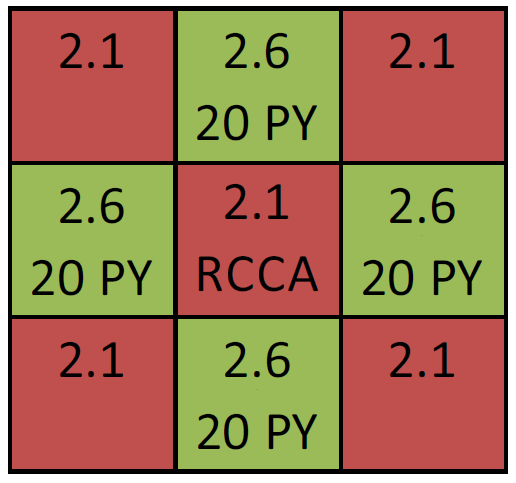
\includegraphics[width=0.4\textwidth]{p4a_layout.png}
}
~
\subfigure{\label{f:p4axial}
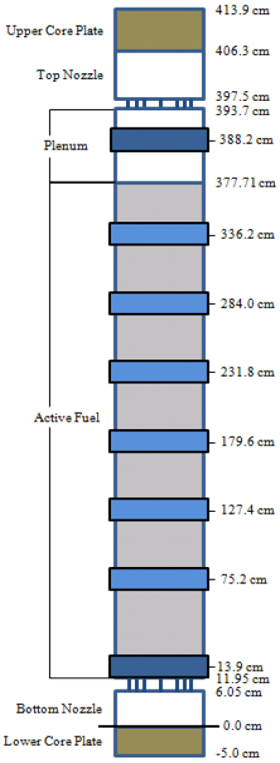
\includegraphics[width=0.3\textwidth]{wb_3d_assembly.png}
}
\caption{VERA Problem 4 radial (a) and axial (b) layouts}\label{f:p4}
\end{figure}

\begin{table}[h]
\centering
\caption{VERA Problem 4 Decusping Results}\label{t:p4decusp}
\resizebox{\textwidth}{!}{
\begin{tabular}{|c|c|c|c|c|c|c|}\hline
\multirow{2}{*}{Case} & k-eff & \multicolumn{2}{|c|}{Pin Power Differences} & \multicolumn{2}{|c|}{Iterations} & Runtime\\\cline{3-6}
 & Difference (pcm) & RMS & Max & 2D/1D & CMFD & (Core-Hours) \\\hline
Reference        & -- & --     & --      & 12 & 517 & 7.81 \\\hline
No Treatment     & -30 & 3.84\% & 21.82\% & 12 & 512 & 8.37 \\\hline
Polynomial       & -7  & 0.95\% &  6.26\% & 12 & 506 & 8.24 \\\hline
Subplane         & -7  & 1.13\% &  7.11\% & 12 & 525 & 8.31 \\\hline
Subplane + 1D-CP & -2  & 0.54\% &  4.96\% & 12 & 526 & 8.37 \\\hline
\end{tabular}
}
\end{table}

The ``No Treatment'' case shows the magnitude of the cusping effects for this problem.  The k$_{eff}$ difference is 30 pcm, which is not too alarming.  However, the RMS and maximum power differences are almost 4\% and over 20\%, respectively, which is an unacceptable level of error.  The polynomial decusping significantly reduces these errors to about 1\% and 6\% respectively.  This is much better, but still quite high.  The sub-plane decusping with no radial treatment performs similarly to the polynomial decusping, but slightly worse.  Because the polynomials were generated using this problem, it is expected that they would perform well.  Thus, the fact that the sub-plane decusping is comparable indicates that it is capturing the axial shape well.  Finally, the CP-based decusping gives the best results, with an RMS of about 0.5\% and a maximum error just under 5\%.  The maximum error is still larger than what is typically desired from the 2D/1D method, but is better than the old decusping treatment and far better than no treatment at all.

As far as runtime is convergence and runtime is concerned, all cases took the same number of 2D/1D iterations.  The sub-plane--based decusping methods incurred a few more CMFD iterations, but this did not have a significant impact on runtime.  The difference in runtime between the reference and no treatment cases is due to the decomposition of the problem.  Both cases use the same sub-plane CMFD mesh (with homogeneous cross-sections in each plane).  However, the reference case was run with 2 MOC planes instead of 1.  This also means that an extra core was used in the calculation.  Because of this, the time required for the transport calculations was the same, but the CMFD solve was slower for the no treatment case since a single core was solving a portion of the CMFD system handled by two cores in the reference calculation.  Thus, the runtime increase is due only to the parallel partitioning, not the methods themselves.  This is important, because the runtimes of the decusping cases were all about the same as the no treatment case.  This implies that the runtime penalty due to the decusping solvers is negligible.  Some work simply needs to be done to improve the parallel balance when using the sub-plane scheme.

\subsection{VERA Problem 5}

To demonstrate the behavior of the decusping methods on a full-core problem, VERA Problem 5 was also run.  Problem 5 is the a beginning-of-cycle simulation of the Watts Bar Unit 1 PWR.  The model of this reactor uses the same axial layout shown in Figure \ref{f:p4axial} with the radial layout shown in Figure \ref{f:p5radial}.  For these calculations, Bank D was set to a position of 257.9 cm above the core plate while all other banks were fully withdrawn.

Like problem 4, the reference case was run with 58 planes while the decusping cases were run with 57 planes.  Radial decomposition was used with 16 cores per MOC plane.  This resulted in a slightly different number of cores for the reference case compared with the others, as seen in the Problem 4 calculations.  The accuracy and convergence data for these calculations is shown in Table \ref{t:p5decusp}.

\begin{figure}[h]
\centering
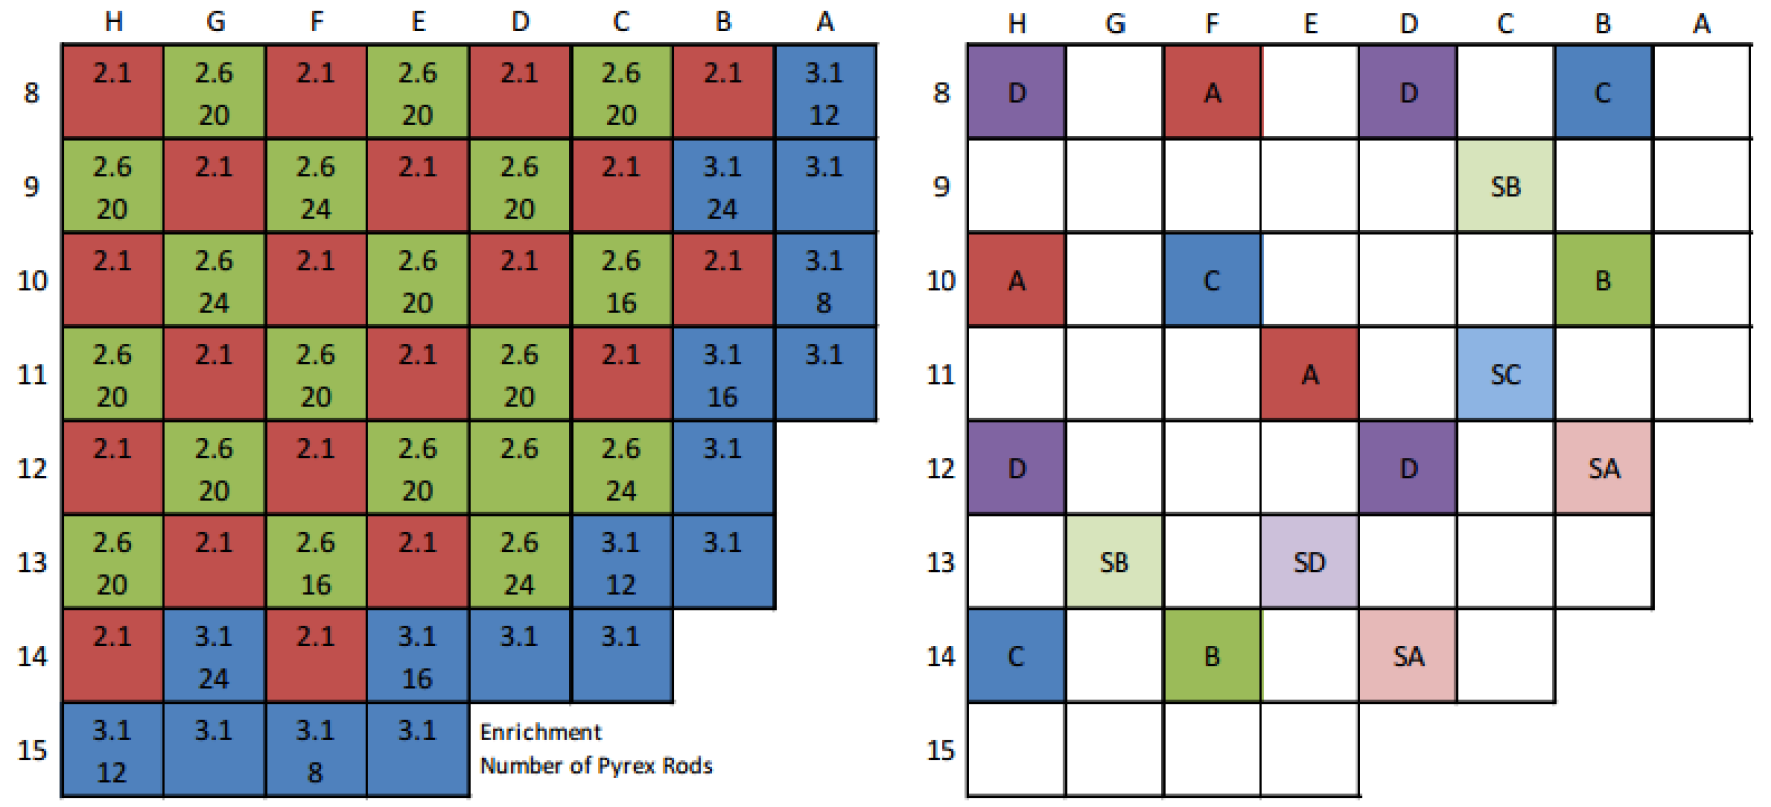
\includegraphics[width=0.9\textwidth]{WB1-cycle1-layout.png}
\caption{VERA Problem 5 radial layout}\label{f:p5radial}
\end{figure}

\begin{table}
\centering
\caption{VERA Problem 5 Decusping Results}\label{t:p5decusp}
\resizebox{\textwidth}{!}{
  \begin{tabular}{|c|c|c|c|c|c|c|}\hline
    \multirow{2}{*}{Case} & k-eff & \multicolumn{2}{|c|}{Pin Power Differences} & \multicolumn{2}{|c|}{Iterations} & Runtime\\\cline{3-6}
    & Difference (pcm) & RMS & Max & 2D/1D & CMFD & (Core-Hours) \\\hline
    Reference        & -- & --     & --      &  &  &  \\\hline
    No Treatment     &  &  &  &  &  &  \\\hline
    Polynomial       &  &  &  &  &  &  \\\hline
    Subplane         &  &  &  &  &  &  \\\hline
    Subplane + 1D-CP &  &  &  &  &  &  \\\hline
  \end{tabular}
}
\end{table}

\hl{Problems are being run now}
%\todo{discussion}